\documentclass[12pt]{article}

\usepackage{graphicx}
\usepackage{float}
\usepackage{svg}
\usepackage{amsmath}
\usepackage{amsfonts} 
\usepackage{hyperref}
\usepackage{color}
\usepackage{pagecolor}
\usepackage[most]{tcolorbox}
\usepackage{tikz}
\usepackage{pgf-pie}
\usepackage{xcolor}


\textheight = 20 cm

\definecolor{blueColor}{HTML}{0069f5}

\begin{document}

\newpage

\pagecolor{blueColor}

\begin{titlepage}
    \centering

     
\includegraphics[width=0.88\textwidth, keepaspectratio]{latex-cover.png}
    
\end{titlepage}

\newpage

\pagecolor{white}

\renewenvironment{abstract}
 {\small
  \begin{center}
  \bfseries \abstractname\vspace{-.5em}\vspace{0pt}
  \end{center}
  \list{}{
    \setlength{\leftmargin}{.5cm}
    \setlength{\rightmargin}{\leftmargin}
  }
  \item\relax}
 {\endlist}
 

\title{\textbf{Pairfy,\\A P2P e-commerce protocol based on trust rating and blind peers }}

\author{Juan C. Rey\footnote{@pairfy  website: \url{www.pairfy.io} - Plutus pioneer first cohort. This personal project was born as a proposal to Y Combinator in 2019 and has been activated for contribution to the open source community.  }\\}

\maketitle

\renewcommand*\abstractname{\textbf{}\hfill}

\abstract{
\textbf{Abstract.}
Pairfy is an electronic commerce protocol that uses smart contracts to decentralize functional requirements necessary for the processes of selling and buying a physical product.
Any member of the community can post a product for sale and any member of the community can express an intention to purchase that product.
The slot of a product is a concept that represents the availability to open a negotiation session similar to a sell order on a DEX. 
A negotiation session is defined as the process of trading a product for a limited time.
During the session the buyer and seller generate the negotiation context by engaging in bilateral communication through live chat via websocket.
If there is a dispute situation during the session it is possible to use the appeal resource so that a group of three mediators decide on the specific case according to the fulfillment of the obligations of the buyer and the seller. The fundamental idea of Pairfy is to avoid using expensive infrastructure and oracles as a source of truth. Instead, use mediators as a source of truth in a disputed negotiation session.

}


\section{Introduction}

Pairfy is an electronic commerce protocol that uses smart contracts to decentralize functional requirements necessary for the processes of selling and buying a physical product.
Any member of the community can post a product for sale and any member of the community can express an intention to purchase that product.
The slot of a product is a concept that represents the availability to open a negotiation session similar to a sell order on a DEX. 
A negotiation session is defined as the process of trading a product for a limited time.
A slot can be released if the buyer or seller cancels the session.
During the session the buyer and seller generate the negotiation context by engaging in bilateral communication through live chat via websocket.
If there is a dispute situation during the session it is possible to use the appeal resource so that a group of three mediators decide on the specific case according to the fulfillment of the obligations of the buyer and the seller.

A completely decentralized e-commerce protocol can be described as trading in physical products or services where parties use digital devices and blockchain to fulfill their obligations.
The seller's obligation is to deliver the product or service and the buyer's obligation is to pay the price corresponding to the product or service. 
The entire process can be digital if the product or service is digital.
Regarding physical products it is necessary to use the service of shipping companies to physical destinations.
To apply blockchain to the physical process of delivering a product it is necessary to establish a digital channel that provides infallible information about the delivery of the product and therefore the fulfillment of the seller's obligation. This can be done by implementing oracles and physical hardware that work together with the blockchain as a source of truth. The fundamental idea of Pairfy is to avoid using expensive infrastructure and oracles as a source of truth. Instead, use mediators as a source of truth in a disputed negotiation session.

\section{ Requirements }

\subsection { Negotiation session }

The negotiation session is a 4-stage synchronous process \emph{Waiting}, \emph{Locking}, \emph{Delivery}, \emph{Finish}. The stages of the session are sequential and not parallel.

\subsubsection { Waiting }

\begin{figure}[ht]
  \centering
  \includesvg[width=0.86\textwidth]{waiting.svg}
  \caption{Script deployment}
  \label{fig:mi_imagen}
\end{figure}


When a seller offers a product to the public by activating a slot (sale order) a small plutus script with state machine logic is activated in the blockchain.
The seller must lock an amount greater than 0 ADA as collateral. 
If the seller acts in bad faith during the negotiation session the seller will lose the collateral.
If the seller is a good agent during the negotiation session the collateral will return to him.
Collateral guarantees that the seller behaves honestly.
This mechanism of coercion allows to generate trust in potential buyers. 
It also allows the seller to increase their trust rating. Example. Alice publishes a book with 20 units of stock.
She activates only 10 slots (sale orders) each with a collateral of 20 ADA.
In the first few hours 7 books were sold and now there are only 3 slots left.
Alice decides to activate the 10 remaining slots due to demand.
Bob sells the same product with the same stock but offers collateral of 5 ADA. The community prefers to buy the books from Alice since she is more committed to fulfilling her obligation by offering 20 ADA collateral.
Other factors increase the seller's trust rating such as the total number of successful sales, seniority, or profile information.
In the background for each activated slot individual scripts are deployed on the blockchain waiting to be occupied by buyers.

\subsubsection { Locking }

\begin{figure}[ht]
  \centering
  \includesvg[width=0.86\textwidth]{locking.svg}
  \caption{Session locked}
  \label{fig:locking}
\end{figure}


In Figure 2 you can see the collateral of 50 ADA given by the seller and the price of the product 100 ADA given by the buyer.
When the buyer presses the buy button a slot is occupied and the state of the script transitions from \emph{Waiting} to \emph{Locking}.
Blocking funds allows participants to advance their obligations.
The seller's obligation is to deliver the correct product with the correct specifications. The buyer's obligation is to receive the product and pay the price.
It is important to clarify that the buyer's obligation to pay the price is guaranteed when he occupies a slot since the amount in ADA of the product price is a necessary condition to occupy a slot.

From this point the seller can start with questions such as: What is the delivery point? Description of delivery point? Any questions necessary to guarantee the effective delivery of the product.

All information provided by both actors in the user interface is contained within a websocket instance and can only be observed by the blind peers in case of a dispute.
The websocket server does not store any type of information about the negotiation session once legal certainty is declared about the business between the parties.
Legal certainty is declared by the blind peers and refers to the absence of reasonable doubt regarding compliance with the obligations that correspond to the buyer and the seller.


\subsubsection { Delivery }


\begin{figure}[ht]
  \centering
  \includesvg[width=0.86\textwidth]{delivery.svg}
  \caption{Delivery confirmed by seller}  
  \label{fig:delivered}
\end{figure}





When the shipping company confirms the effective delivery of the product the seller can invoke the @delivered endpoint.
The script transitions from \emph{Locking} to the \emph{Delivery} state which indicates that the seller has fulfilled its delivery obligation.
Finally, the buyer confirms whether he received the product by invoking the @received endpoint. By doing so, the script transitions to the last state \emph{Finish} which releases the funds to the seller's wallet.


\subsubsection { Finish }

\begin{figure}[ht]
  \centering
  \includesvg[width=0.86\textwidth]{finish.svg}
  \caption{Delivery confirmed by buyer}
  \label{fig:delivered}
\end{figure}

The seller receives 50 ADA of collateral and 100 ADA equivalent to the price of the product he sold to the buyer.
\\
\\
\\
\\
\\
\\
\\
\\
\\
\\
\\
\\
\\
\\
\\
\\
\\

\subsubsection { State machine }
A state machine also known as a finite state machine (FSM), is a mathematical model used to describe the behavior of a system or process that can exist in a limited number of distinct states. The system transitions from one state to another in response to specific events or input conditions and these transitions are defined by a set of rules or conditions known as transitions.

A deterministic finite state machine (DFSM) is a specific type of state machine that exhibits deterministic behavior, meaning that for any given state and input there is a unique and unambiguous next state. In a deterministic state machine, the transition from one state to another is uniquely determined by the current state and the input with no ambiguity or randomness involved.

Figure 5 shows the deterministic state machine concepts applied to the steps of a negotiation session. 
The EUTXO model of the Cardano blockchain implies that smart contracts need an initial transaction for their logic to be activated and establish their initial state.
When the seller activates a slot his wallet deploys a plutus script that receives the collateral in ADA and necessary parameters for the session. 

\begin{figure}[ht]
  \centering
  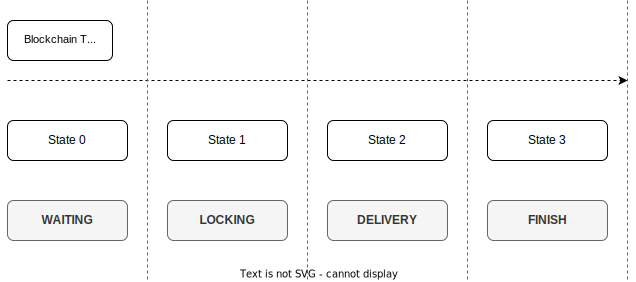
\includegraphics[width=0.95\textwidth]{machine.png}
  \caption{Session states}
  \label{fig:States}
\end{figure}


\begin{tabular}{lr}
\textbf{sessionState} \emph{:: SessionState}\\
\textbf{sessionState}  = SessionState  \textbraceleft{}
\\ \hspace{54mm}cState = 0
\\ \hspace{54mm}sLabel = ``waiting"
\\ \hspace{54mm}tDuration = 100
\\ \hspace{54mm}bSlot = False
\\ \hspace{54mm}pDelivered = False
\\ \hspace{54mm}pReceived = False
\\\hspace{51mm}\textbraceright{} 
\end{tabular}
\\

 The data type \emph{sessionState} represents the initial state of the plutus script once deployed by the seller. These variables will remain in the default state indefinitely until the buyer's wallet interacts with the script taking the slot.
\\

\begin{tabular}{lr}
\textbf{sessionState} \emph{:: SessionState}\\
\textbf{sessionState}  = SessionState  \textbraceleft{}
\\ \hspace{54mm}cState = 1
\\ \hspace{54mm}sLabel = ``locking"
\\ \hspace{54mm}tDuration = 100
\\ \hspace{54mm}bSlot = True
\\ \hspace{54mm}pDelivered = False
\\ \hspace{54mm}pReceived = False
\\\hspace{51mm}\textbraceright{} 
\end{tabular}
\\

 \emph{bSlot} represents the variable that indicates whether the script has been occupied by a buyer. The boolean value True means that the slot has been occupied by a buyer which makes the script transition from \emph{Waiting} to \emph{Locking}.
\\

\begin{tabular}{lr}
\textbf{sessionState} \emph{:: SessionState}\\
\textbf{sessionState}  = SessionState  \textbraceleft{}
\\ \hspace{54mm}cState = 2
\\ \hspace{54mm}sLabel = ``delivery"
\\ \hspace{54mm}tDuration = 100
\\ \hspace{54mm}bSlot = True
\\ \hspace{54mm}pDelivered = True
\\ \hspace{54mm}pReceived = False
\\\hspace{51mm}\textbraceright{} 
\end{tabular}
\\

\emph{pDelivered} is a variable of type boolean that represents the delivery of the product or not. 
At this point the seller has invoked the @delivered endpoint stating that he has fulfilled his obligation to deliver the product. This action makes the script transition from \emph{Locking} to \emph{Delivery}
\\

\begin{tabular}{lr}
\textbf{sessionState} \emph{:: SessionState}\\
\textbf{sessionState}  = SessionState  \textbraceleft{}
\\ \hspace{54mm}cState = 3
\\ \hspace{54mm}sLabel = ``finish"
\\ \hspace{54mm}tDuration = 100
\\ \hspace{54mm}bSlot = True
\\ \hspace{54mm}pDelivered = True
\\ \hspace{54mm}pReceived = True
\\\hspace{51mm}\textbraceright{} 
\end{tabular}
\\

\emph{pReceived} is a boolean variable that represents whether the buyer confirms receipt of the product or not. This variable is modified only by the buyer using the @received endpoint.
By doing this, the script transitions to its final state \emph{Finish} which releases the funds to the seller.
 
\subsection { Blind peers }  

Connecting the blockchain to the real world is an expensive challenge at least for trading physical products.
Shipping companies would have to connect their vehicles to supervised oracles and the products must have an infallible tracker to check if were delivered.
A lot of infrastructure deployed around the world is necessary to achieve a fully decentralized ecommerce protocol.
Clearly this represents a very difficult challenge to achieve in contrast to another option which is to use the human brain as a source of truth.
With the right conditions the human brain can make logical reasoning about facts or propositions to declare a truth.
For example, the peer review system in the academic world allows a research paper to be reviewed by randomly assigned experts.
A blind reviewer does not know who is the author of the paper he is reviewing and the author also does not know who the reviewers are.
The system maintains confidentiality to prevent biases, ensuring a rigorous and impartial assessment. Serving as a crucial quality control mechanism, it identifies errors, provides constructive feedback to authors and contributes to the overall accuracy and reliability of published work. 
A system of blind peers trained in conflict resolution can decide on a dispute in a negotiation session in the event that the buyer or seller fails to comply with their obligations or another problem arises that does not allow the natural conclusion of the session.
A blind peer system can decide on a disputed trading session.

Some characteristics of the profile of a mediator are:

1. Mediators must stay neutral and impartial to ensure a fair and unbiased assessment of disputes fostering trust in the mediation process for all parties involved.

2. Effective communication is vital for mediators, involving active listening, skillful facilitation of discussions and clear conveyance of information to aid parties in mutual understanding and resolution.

3. A mediator needs strong problem-solving skills to navigate complex disputes and find mutually acceptable solutions. 

4. Mediators require patience as mediation processes take time, allowing parties to express themselves, explore solutions and reach agreements at their own pace.

5. Mediators must uphold ethical standards ensuring the confidentiality of the mediation process to establish and maintain the crucial element of trust for successful resolution.

6. Mediators require a comprehensive skill set encompassing technical, legal, and cultural knowledge to effectively carry out their duties.

\subsubsection { Appeal } 

\emph{Peer-to-Peer} cryptocurrency exchange services such as localbitcoins or binance P2P have proven to be systems that work for secure trades. These systems are based on trust rating and involve real-world action on the part of the buyer such as making a transaction to the bank account provided by the seller. In Binance P2P, disputes between buyers and sellers can be addressed through an appeal process. Common reasons for initiating an appeal involves problems with payment confirmation, disagreements over payment quality, or disputes regarding trade terms. To protect the cryptocurrency involved in the trade an escrow system locks the funds.

Both the buyer and seller are afforded the opportunity to present evidence or explanations supporting their case during the appeal. A mediation team at Binance reviews the appeal carefully considering the evidence and arguments put forth by both parties. Subsequently, Binance reaches a decision which may involve upholding the original trade agreement, releasing funds from escrow to the appropriate party, or taking other actions based on the specific circumstances of the dispute.

In the case of Pairfy the seller is the party that has control over the terms of the negotiation. The UI view of a published product contains the product description, seller name, seniority, trust rating, number of successful sales, number of total sales, and the terms that any buyer must meet to be able to negotiate with the seller. These terms must be clear, enumerated and determined. Any buyer who accepts the seller's terms must comply with them.

It is not convenient for the seller to use the @delivered endpoint if he has not fulfilled his obligation since he has to prove it to a level of certainty at the risk of losing his collateral. The seller also cannot use the endpoint by mistake since the user interface would have mechanisms to prevent this. It is also not convenient for the buyer to use the @received endpoint without having received the product since he would lose the funds corresponding to the price. He also cannot do it by mistake since the UI does not allow it.

If the buyer does not comply with his obligation to receive the product, the seller can initiate the appeal. If the intention of abuse is proven, then the buyer loses the equivalent of the collateral proposed by the seller. Both parties can resort to appeal in case of dispute, a group of blind mediators can take action on a case-by-case basis.

\subsubsection { Pool } 

According to the principle of least cardinality in data modeling which states that one-to-many relationships such as between the author and the $N$ of published posts, the identifier that relates them should be stored on the ``many" side. In other words, when data modeling is designed posts should store the author identifier, authors should not store identifiers about their posts. As long as the author has a small number of published posts there are no problems with storing and consulting the information. The problem arises when the author has a large number of published posts, the storage of post identifiers in one of the author variables represents a scaling problem and the query time can be affected.
The application of this principle in the protocol architecture allows high horizontal scalability.
Pairfy uses a master-slave pattern in which the master is the main contract of the protocol which manages the pool of mediators.
Slaves are the individual scripts that are in charge of the trading sessions. For each activated slot of a product a script is deployed waiting to be occupied by a buyer.


\begin{figure}[ht]
  \centering
  \includesvg[width=0.86\textwidth]{contract.svg}
  \caption{Pairfy instances}
  \label{fig:delivered}
\end{figure}


Figure 6 shows a grouping of consecutive contracts representing horizontal scaling to ensure high concurrency and availability of the Pairfy service.
When a seller enables a product slot a slave script with state machine logic is deployed in the blockchain waiting for a buyer to occupy it to start a negotiation session.
Each slave script has by default the \emph{PubKeyHash} of the master contract in its datum.
A slave cannot interact with another contract other than its master.

Master contracts do not have any information about their slaves, their function is to provide mediation service in case of a dispute during a negotiation session by enabling an endpoint called @appeal. The endpoint is designed to be used by slave scripts and requires an ADA fee to prevent abuse.


The mediator pool is basically a set of \emph{PubKeyHash} each corresponding to the wallet of a certified and active mediator. 
When @appeal is triggered by a slave the master contract mint an NFT and within the NFTdatum the contract adds three (3) \emph{PubKeyHash} contained in the pool of mediators.
Subsequently the contract removes those three \emph{PubKeyHash} from the pool queue.

The slave receives the NFT and adds to its own datum the three \emph{PubKeyHash} that are within the NFTdatum. After this process the slave has exact information about the mediators authorized to decide on the current dispute. Mediators are the only ones who can activate special @endpoints of the slave to decide the dispute.


\subsubsection { Designation } 

The community using governance can change the policies and parameters of the protocol. The community can also decide who meets the characteristics to be a mediator or not.
Mediators can have two states: active and inactive.
Only active mediators can enter the pool.

\subsubsection { Rewards } 

To avoid bias and inactivity mediators are rewarded every 30 days with utility token. The amount will be decided by community governance. Only active days in the pool can be rewarded.

\subsubsection { Penalties } 

To avoid bias and inactivity mediators are rewarded every 30 days with utility token. The amount will be decided by community governance. Only active days in the pool can be rewarded.

\subsection{ User interface }

\subsubsection { Product } 

Any member of the community can publish a product only if they meet the following conditions:

1. Cannot be published any object, substance, biological, physical matter in any of its states and forms, declared illegal or prohibited by any type of international, state, federal, local or other regulations on the subject.

2. Comply with international, state, federal, local or other regulations on money laundering and drug trafficking.

3. Only physical products can be published, publication of services is not allowed.

4. Know and understand the licenses associated with the product.

5. Write in a specific and enumerated way the terms and conditions that the buyer must comply with.

6. Product must meet safety standards, must not pose a threat to the health or safety of the consumer.

7. Buyer have the right to be informed about the terms and conditions of a transaction, warranties, and return policies.

8. Comply with all international, state, federal, local and any regulations that regulate intellectual property rights.

9. Description of the product in a determined, fair, exact and precise manner.

10. Send the product with a recognized shipping company that allows tracking service.

In the user interface the product view must have the name of the product, the description of the product, the terms of the seller, the number of total sales of the seller, the number of successful sales of the seller, information about the seller, the stock number of the product, the number of activated slots, amount of ADA as collateral and trust rating. In the backend of the protocol there must be an automated service in charge of verifying the products before they are visible to the community.


\subsubsection { Session } 

When a buyer presses the buy button on a product publication the website redirects them to a single page. The view of a negotiation session contains all the information corresponding to the product, about the seller, the terms of sale, the appeal button, buttons to upload attached images as evidence, alert indications and for the user experience. It also contains live chat to establish bilateral communication between the parties and the mediators.

\subsubsection { Mediators } 

Mediators assigned to a disputed negotiation session will have a special section in the live chat to communicate with the buyer and the seller at the same time. The mediators have no knowledge about the seller and the buyer because they are shown as anonymous digital entities. Mediators cannot be identified by their wallet addresses because they are dynamic addresses changed by the backend.




\end{document}
